\documentclass[10pt,letterpaper]{article}
\usepackage[left=0.25in,right=3.25in,top=0.6in,bottom=0.6in]{geometry}
\usepackage[T1]{fontenc}
\usepackage{lmodern,amsmath,amssymb,booktabs,tabularx,longtable,graphicx,enumitem}
\usepackage[round,authoryear]{natbib}
\usepackage[colorlinks=true,urlcolor=blue,citecolor=blue,linkcolor=blue]{hyperref}
\usepackage{eso-pic,tikz,microtype,placeins}
\setlength{\parindent}{0pt}
\setlength{\parskip}{5pt}
\setlist{nosep,leftmargin=*}
\AddToShipoutPictureBG{%
  \AtPageLowerLeft{\begin{tikzpicture}[overlay,x=1in,y=1in]
    \draw[red!25,line width=0.35pt] (5.32,0.6)--(5.32,10.4);
    \foreach \k in {0,...,34} {
      \draw[blue!19,line width=0.3pt] (5.4,{0.6+0.28125*\k})--(8.25,{0.6+0.28125*\k});
    }
  \end{tikzpicture}}}
\newcommand{\C}{\,^\circ\mathrm{C}}
\newcommand{\pending}[1]{\textit{Pending final checked calculation: #1.}}
\title{\vspace{-1.3em}TC-Lab: an $n=1$ teaching study\\\large Tiers 0--2, researcher review draft}
\author{Prepared for Alex Dowling}
\date{October 24, 2026}
\begin{document}
\maketitle
\vspace{-1em}
\begin{tabularx}{\linewidth}{@{}p{0.38in}X p{1.35in}@{}}
\toprule
Tier & Goal & Status and result\\
\midrule
0 & Test whether one shared thermal model explains all twelve ENV2 records. Diagnose ambient treatment and residual covariance. & Fits complete. Shared-model adequacy remains unresolved.\\
1 & Fit one five-minute sine and one step. Quantify uncertainty and predict the other ten records. & Point fit complete; uncertainty and evaluation pending.\\
2 & Repeat with five further pairs, balancing three steps and three sine periods. & Six total point fits complete; uncertainty and evaluation pending.\\
3 & Consider the remaining one-sine/one-step combinations after review. & Deferred for Alex's feedback.\\
\bottomrule
\end{tabularx}

\textbf{Current interpretation.} P1 gives narrow thermal parameter ranges but transfers poorly to the other ten records. Its zero-ambient predictions have pooled RMSE $2.22\C$, and 19.0\% of recorded temperatures fall inside the nominal 95\% Gaussian observation ranges. Allowing the $\pm2\C$ ambient envelope raises that fraction to 58.5\%. The pooled residual analysis also retains a command-related cycle in the thirty-second sine records. These findings limit the proposed universal mean/error description. The uncertainty calculations remain conditional on that working description and its resampling sensitivities.

\section{Model, records and teaching sequence}
We accept the same-device ENV2 provenance as the study assumption. There are nine sine records (three runs each at 30, 120 and 300 seconds) and three step records. Calibration aliases with duplicate data are excluded.

For experiment $j$, the measured command $u_j$ is held constant from its recorded timestamp to the next update. We propagate the two-state model exactly:
\begin{align}
\theta\dot z_j &= u_j-z_j,\\
\tau\dot T_j &= -T_j+T_{\mathrm{amb},j}+Kz_j,\\
T_{\mathrm{amb},j} &= T_{1,j}(0)+\delta_j,\qquad -2\C\leq\delta_j\leq2\C.
\end{align}
The positive $K,\tau,\theta$ are shared across calibration records. The initial conditions are $z_j(0)=0$ and $T_j(0)=T_{1,j}(0)$; the first temperature is conditioned on and its residual omitted. Initial temperature is a reference, not an independent ambient measurement. The drift comparison replaces the constant correction by a linear function with both endpoints inside the same band. Endpoint bounds are an implementation choice.

The input-lag state is one stage of the delay chain; it produces a first-order lag rather than an exact dead time. Numerical fit bounds are $K\in[0.2,1.5]\C/\%$, $\tau\in[5,600]$ s and $\theta\in[0.01,200]$ s. These are declared computational choices, not measured physical limits. A finite-box profile alone cannot prove global identifiability.

With a fixed command-to-power conversion $c$, a lumped physical interpretation is $K=\alpha c/(UA)$ and $\tau=C_p/(UA)$. An unknown shared constant $\alpha$ is absorbed into fitted $K$. Estimating $\alpha$ separately adds no temperature-fit flexibility when $K$ is free. Independent calibration is needed to recover absolute $UA$ or $C_p$; it is not needed to fit $K$.

The cold, zero-offset command transfer is
\[
G(s)=\frac{K}{(1+\tau s)(1+\theta s)}.
\]
Its two poles can be exchanged without changing that response. The assumed ambient channel acts through $\tau$, so a nonzero offset can distinguish labels conditionally on that channel. We retain both optimization basins and report unlabeled slow/fast poles where useful; pole labels alone do not establish heater or sensor constants.

The teaching sequence is: fit the mean, inspect residuals, fit their temporal covariance, transform response and sensitivities, refit, then reassess uncertainty and predictions. A diagonal set of weights cannot remove temporal correlation.

\section{Tier 0: pooled structure exploration}
\textbf{Goal.} Determine whether one shared $n=1$ description explains all twelve runs, and use discrepancies to assess ambient drift and error structure.

\begin{tabular}{@{}lrrr@{}}
\toprule
Ambient treatment & RMSE, $\C$ & SSE reduction & At bounds\\
\midrule
Constant offset & 0.46574 & --- & 7/12\\
Linear endpoints & 0.43702 & 11.95\% & 9/12\\
\bottomrule
\end{tabular}

These are ordinary least-squares fits. Their raw residual lag-one correlations remain 0.879--0.966 for constant offsets. The training reduction from drift does not settle the ambient question.

We compared IID, Ornstein--Uhlenbeck (OU), OU plus independent measurement noise, and Mat\'ern-$3/2$ plus measurement noise under both ambient treatments. Each cell used 24 starts and an alternating generalized-least-squares (GLS) fit. Independent dense-covariance reconstruction checked all 96 selected run trajectories and likelihoods. Alternating GLS and joint likelihood agree within $1.2\times10^{-6}$ in negative log likelihood.

\begin{tabularx}{\linewidth}{@{}Xrr@{}}
\toprule
Constant-offset error model & Raw RMSE, $\C$ & Innovation lag-one range\\
\midrule
IID & 0.46574 & 0.879 to 0.966\\
OU & 0.46709 & $-0.541$ to $-0.307$\\
OU + measurement noise & 0.48320 & $-0.239$ to 0.238\\
Mat\'ern-$3/2$ + measurement noise & 0.47981 & $-0.186$ to 0.241\\
\bottomrule
\end{tabularx}

The working choice is constant offsets and OU plus measurement noise. Its pooled estimates are $K=0.71001\C/\%$, $\tau=137.48$ s, $\theta=18.37$ s and correlation length $\ell=213.87$ s. The total marginal residual SD is $0.47877\C$, split into $0.47012\C$ slow variation and $0.09062\C$ independent measurement variation. Correlated likelihood emphasizes a different part of the residual spectrum than OLS, so a larger raw RMSE can accompany a better likelihood.

This working choice is agent-selected for the requested six-pair analysis and awaits Alex's scientific review. OU alone leaves strongly negative lag-one innovations; adding measurement variance reduces that effect. The remaining cycle still needs a mean-model explanation or a better disturbance model.

With the same covariance family, linear drift lowers negative log likelihood by 6.05 while adding twelve parameters; nominal AICc is 12.00 higher than for constant offsets. This is a conditional comparison under an imperfect error model.

\begin{figure}[htbp]
\centering
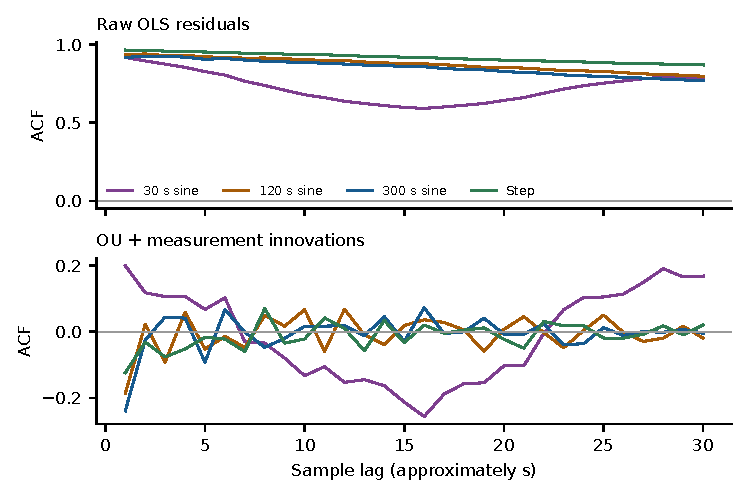
\includegraphics[width=\linewidth]{generated_release/figures/residual_ACF.pdf}
\caption{Residual correlation before and after the covariance-aware fit, using run 1 of each protocol. Whitening reduces the long persistence but leaves oscillation in the thirty-second sine and negative short-lag association in other records. These are descriptive ACFs; no IID significance bands are implied.}
\end{figure}

\subsection*{What remains in the residuals}
The thirty-second sine runs have maximum absolute innovation/command correlations of 0.457--0.481 over the declared $\pm30$-sample lag search. Widening ambient offsets to $\pm4\C$, changing startup by $\pm0.165\C$, adding one second of input prehistory, or using linear ambient drift leaves this cycle. Right-held commands worsen negative log likelihood by 256.30 and increase that association.

The temperatures lie on an inferred $0.32229984\C$ grid after two-decimal reporting. A rounding sensitivity can reproduce some negative innovation correlation. It does not reproduce the command association. We generated and fully refitted 200 Gaussian and 200 rounded-measurement records from the pooled model. Neither mechanism reaches the observed maximum correlation of 0.481; their simulated 99th percentiles are 0.113 and 0.110. These plug-in diagnostic simulations challenge the working model; they do not identify the missing mechanism.

Ambient assumptions also affect interpretation. Widening offsets to $\pm4\C$ removes active ambient bounds and lowers $K$ by 2.47\%, while the fast-sine discrepancy persists. Protocol-specific exploratory fits give $K=0.655,0.689,0.724,0.753$ for 30-second, 120-second, 300-second and step records. Those fits use different observations, so their likelihoods are not directly comparable and the point differences are not a formal heterogeneity test.

\FloatBarrier
\section{Tier 1: one sine and one step}
\textbf{Goal.} Freeze the working structure, refit all numerical thermal, ambient and noise parameters using only five-minute sine run 1 and step run 1, then predict the other ten records.

The P1 point estimates are $K=0.74063\C/\%$, $\tau=147.60$ s and $\theta=16.59$ s. Its two ambient corrections are $1.261\C$ and $1.947\C$. No pooled noise estimate is fixed in this restricted fit.

\begin{center}\small
\begin{tabularx}{\linewidth}{@{}l>{\raggedleft\arraybackslash}X>{\raggedleft\arraybackslash}X>{\raggedleft\arraybackslash}X>{\raggedleft\arraybackslash}X@{}}
\toprule
Parameter & IID SD & HAC(30) SD & GLS SD & Full-curvature SD\\
\midrule
$K$ & 0.0008118 & 0.003714 & 0.005981 & 0.00598\\
$\tau$ & 0.1453 & 0.6578 & 1.235 & 1.232\\
$\theta$ & 0.04781 & 0.2226 & 0.288 & 0.286\\
\bottomrule
\end{tabularx}
\end{center}
SD units are $\C/\%$ for $K$ and seconds for the time constants. HAC changes the estimated OLS covariance while retaining its mean fit. IID and GLS use their own fitted means; their comparison includes the change in fitting criterion. GLS holds the covariance fixed. Full curvature includes noise estimation but remains a local, single-basin diagnostic.
\begin{center}\small
\begin{tabularx}{\linewidth}{@{}l>{\raggedleft\arraybackslash}X>{\raggedleft\arraybackslash}X@{}}
\toprule
Parameter & Gaussian 95\% range & Block 95\% range\\
\midrule
$K$ & [0.737, 0.757] & [0.737, 0.753]\\
$\tau$ & [145.900, 150.008] & [145.756, 150.088]\\
$\theta$ & [16.093, 17.266] & [15.947, 17.202]\\
\bottomrule
\end{tabularx}
\end{center}
Bootstrap refits include noise and ambient estimation, boundaries and pole alternatives. Percentile ranges summarize the working refit distributions; coverage has not been established.
The opposite pole labeling occurs in 8/400 Gaussian and 3/400 block refits. A central interval can miss that secondary basin. The step ambient bound is active in 162/400 Gaussian refits.
Nominal profile support is $K$: [0.7361, 0.7533]; $\tau$: [145.7, 150.2]; $\theta$: [16.02, 17.14]. Finite grid and crossing brackets are retained in the numerical archive.
\begin{figure}[htbp]\centering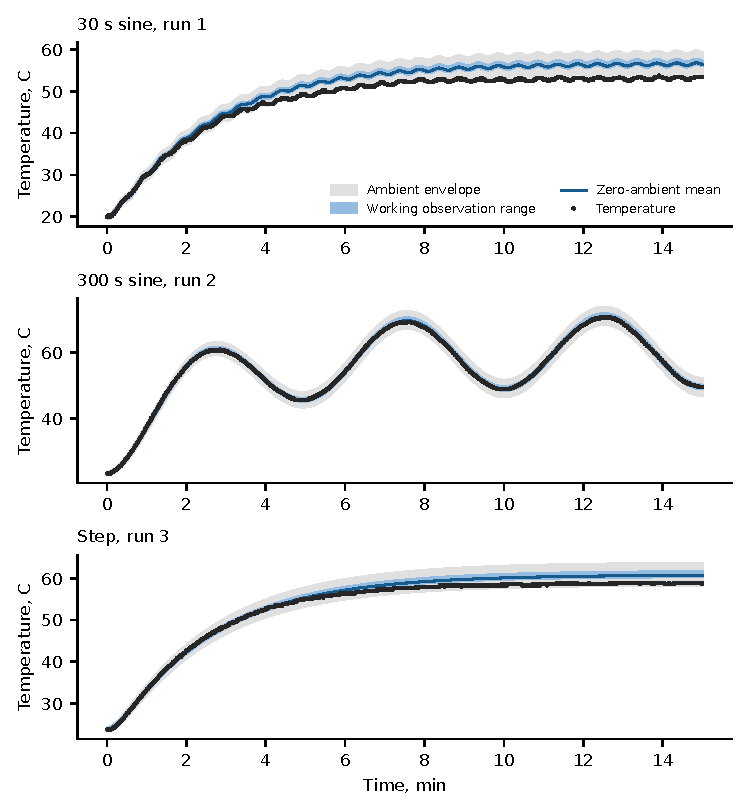
\includegraphics[width=\linewidth]{generated_release/figures/P1_predictions.pdf}\caption{P1 predictions for three evaluation records. Blue bands are pointwise Gaussian working observation ranges at zero future ambient correction; gray envelopes also allow ambient offsets in $\pm2\C$. Ambient envelopes have no assigned probability. Black points are recorded temperatures.}\end{figure}

\FloatBarrier
\section{Tier 2: five further pairs}
\textbf{Goal.} Assess how much the result depends on the chosen sine and step. Six pairs in total use each step twice and each sine period twice.

\begin{tabular}{@{}llrrrr@{}}
\toprule
Pair & Sine (period/run) & Step run & $K$, $\C/\%$ & $\tau$, s & $\theta$, s\\
\midrule
P1 & 300 s / 1 & 1 & 0.74063 & 147.60 & 16.59\\
P2 & 30 s / 2 & 1 & 0.71402 & 127.70 & 22.17\\
P3 & 120 s / 1 & 2 & 0.72390 & 137.22 & 18.47\\
P4 & 300 s / 3 & 2 & 0.72193 & 146.61 & 16.12\\
P5 & 30 s / 3 & 3 & 0.67651 & 129.75 & 19.57\\
P6 & 120 s / 2 & 3 & 0.69734 & 130.62 & 18.87\\
\bottomrule
\end{tabular}

All six point fits pass the declared stationarity checks and independent trajectory/likelihood reconstruction. Their parameter spread can reflect record variation, nuisance-bound effects and model inadequacy as well as statistical uncertainty.
\begin{center}\small
\begin{tabularx}{\linewidth}{@{}l>{\raggedleft\arraybackslash}X>{\raggedleft\arraybackslash}X>{\raggedleft\arraybackslash}X@{}}
\toprule
Pair & Gaussian $K$ range & Block $K$ range & Swaps G/B\\
\midrule
P1 & [0.737, 0.757] & [0.737, 0.753] & 8/3\\
P2 & [0.691, 0.733] & [0.698, 0.728] & 21/10\\
P3 & [0.707, 0.736] & [0.711, 0.737] & 1/1\\
P4 & [0.718, 0.738] & [0.721, 0.739] & 1/2\\
P5 & [0.661, 0.705] & [0.661, 0.707] & 0/0\\
P6 & [0.686, 0.702] & [0.688, 0.702] & 0/0\\
\bottomrule
\end{tabularx}
\end{center}
G/B counts use 400 draws per method. They are bootstrap selection frequencies under the working mechanism, not posterior probabilities of a physical pole assignment.
\begin{center}\small
\begin{tabularx}{\linewidth}{@{}l>{\raggedleft\arraybackslash}X>{\raggedleft\arraybackslash}X@{}}
\toprule
Pair & Unlabeled slow pole, s & Unlabeled fast pole, s\\
\midrule
P1 & [146.1, 150.7] & [16.1, 17.1]\\
P2 & [117.5, 138.7] & [19.6, 24.6]\\
P3 & [132.8, 140.6] & [17.9, 19.0]\\
P4 & [144.9, 150.4] & [15.5, 16.7]\\
P5 & [127.6, 131.8] & [18.3, 20.9]\\
P6 & [129.3, 132.0] & [18.3, 19.3]\\
\bottomrule
\end{tabularx}
\end{center}
These are Gaussian percentile ranges. Unlabeled poles avoid combining two swapped parameter basins in a single interval for a physical time constant.
\begin{center}\small
\begin{tabularx}{\linewidth}{@{}l>{\raggedleft\arraybackslash}X>{\raggedleft\arraybackslash}X>{\raggedleft\arraybackslash}X@{}}
\toprule
Pair & $K$ width: 30-s blocks & 60-s blocks & 120-s blocks\\
\midrule
P1 & 0.0147 & 0.0152 & 0.0163\\
P2 & 0.0293 & 0.0298 & 0.0481\\
P3 & 0.0257 & 0.0265 & 0.0215\\
P4 & 0.0215 & 0.0183 & 0.0180\\
P5 & 0.0447 & 0.0455 & 0.0460\\
P6 & 0.0148 & 0.0141 & 0.0127\\
\bottomrule
\end{tabularx}
\end{center}
Widths are in $\C/\%$. Blocks count samples, approximately seconds. The 30/120-s sensitivities use 100 draws each; their 2.5\% tails involve only two or three order statistics. The 400-draw primary methods have about ten draws per tail. Rare pole switches can move endpoints; the archive retains order-statistic Monte Carlo ranges and half-batch discrepancies.
\begin{center}\small
\begin{tabularx}{\linewidth}{@{}l>{\raggedleft\arraybackslash}X>{\raggedleft\arraybackslash}X>{\raggedleft\arraybackslash}X@{}}
\toprule
Pair & Smallest information eigenvalue & Condition & Weak log direction\\
\midrule
P1 & 2.77e+03 & 43.8 & (-0.26, -0.36, 0.89)\\
P2 & 191 & 10.5 & (0.13, -0.49, 0.86)\\
P3 & 2.04e+03 & 22.3 & (0.54, 0.72, -0.44)\\
P4 & 1.5e+03 & 53.8 & (-0.33, -0.42, 0.84)\\
P5 & 791 & 62.1 & (-0.46, -0.11, 0.88)\\
P6 & 5.28e+03 & 15.5 & (0.26, -0.24, 0.94)\\
\bottomrule
\end{tabularx}
\end{center}
Directions use $(\log K,\log\tau,\log\theta)$ after eliminating ambient columns; eigenvector signs are arbitrary. These are local fixed-covariance diagnostics and ignore box geometry and separated modes.
All six conditional thermal information matrices have rank three at relative eigenvalue thresholds $10^{-8}$, $10^{-10}$ and $10^{-12}$. P2's full observed curvature is indefinite, so its regular Gaussian covariance is withheld. P4 has an active ambient bound despite positive observed curvature. Rank and positive curvature alone do not settle bounded or global inference.
\begin{center}\small
\begin{tabularx}{\linewidth}{@{}l>{\raggedleft\arraybackslash}X>{\raggedleft\arraybackslash}X>{\raggedleft\arraybackslash}X>{\raggedleft\arraybackslash}X@{}}
\toprule
Pair & OLS RMSE & GLS RMSE & Common sines & Ambient reconstruction\\
\midrule
P1 & 2.175 & 2.219 & 2.168 & 0.930\\
P2 & 1.605 & 1.695 & 1.736 & 0.606\\
P3 & 2.038 & 1.950 & 1.831 & 0.629\\
P4 & 1.881 & 1.881 & 1.625 & 0.576\\
P5 & 1.853 & 2.223 & 1.431 & 1.085\\
P6 & 1.856 & 1.856 & 1.358 & 0.684\\
\bottomrule
\end{tabularx}
\end{center}
RMSE is in degrees Celsius. OLS/GLS columns pool each pair's ten evaluation records; the exclusions differ, so those aggregates are not a controlled same-test-set ranking. Common sines restrict GLS evaluation to 30-s run 1, 120-s run 3 and 300-s run 2, which are excluded from all six calibrations. Primary predictions use zero future ambient correction. The last column fits an offset using the complete evaluation response and is retrospective reconstruction.
\begin{center}\small
\begin{tabularx}{\linewidth}{@{}l>{\raggedleft\arraybackslash}X>{\raggedleft\arraybackslash}X>{\raggedleft\arraybackslash}X@{}}
\toprule
Pair & Gaussian inside, \% & Block inside, \% & Gaussian + ambient, \%\\
\midrule
P1 & 19.0 & 20.5 & 58.5\\
P2 & 55.3 & 43.6 & 100.0\\
P3 & 32.9 & 29.3 & 89.8\\
P4 & 16.8 & 20.0 & 73.1\\
P5 & 50.8 & 54.2 & 80.7\\
P6 & 15.7 & 14.8 & 79.0\\
\bottomrule
\end{tabularx}
\end{center}
Fractions count measured temperatures inside pointwise future-observation ranges, pooled by sample count. Ambient envelopes are scenarios. Overlapping evaluation records and serial dependence prevent independent-binomial coverage claims.
\begin{figure}[htbp]\centering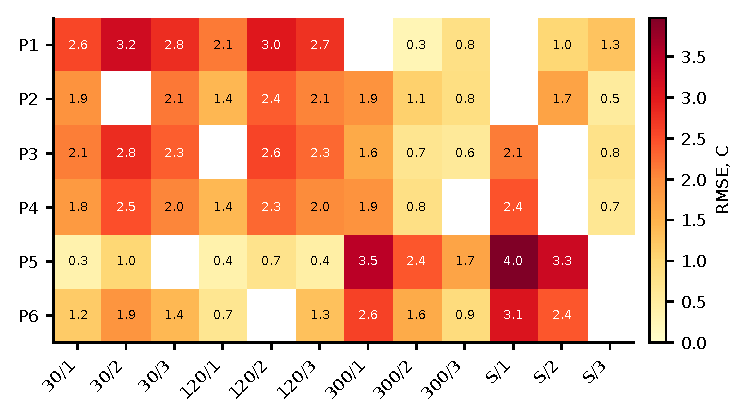
\includegraphics[width=\linewidth]{generated_release/figures/prediction_RMSE.pdf}\caption{Zero-ambient prediction RMSE in degrees Celsius. White cells are the two calibration records for that pair. Records are labeled by sine period or step (S), then run number.}\end{figure}

\FloatBarrier

\section{How uncertainty is calculated}
For $e_j=y_j-m_j$, the working covariance is
\[
C_j=\sigma^2 R_j,\qquad
(R_j)_{ab}=(1-\eta)e^{-|t_a-t_b|/\ell}+\eta\,\mathbf1_{a=b}.
\]
Here $\eta$ is a variance fraction. A stationary innovations filter provides $W_j$ with $W_jR_jW_j^\mathsf T=I$. We transform the response and every design column. For fixed nonlinear coordinates we solve bounded least squares for gain and ambient corrections, profile $\sigma^2=\sum_j\|W_je_j\|^2/N$, and minimize
\[
-\log L=\tfrac12\left[N\{\log(2\pi)+1+\log(\widehat\sigma^2)\}
+\sum_j\log|R_j|\right].
\]
The determinant is required when estimating covariance parameters. State-space representations of half-integer Mat\'ern kernels support exact temporal covariance computations with stationary initialization and irregular sampling \citep{hartikainen-2010-kalman}. They provide a computation method, not evidence that a chosen kernel describes these experiments.

The declared covariance search uses $\ell\in[0.05,3000]$ s and $\eta\in[0,1]$. Processes reset independently between experiments. Alternating GLS updates covariance from the current residuals, refits the transformed mean, and repeats; joint likelihood then checks the stabilized solution.

Local information uses log $K,\tau,\theta$, removes ambient directions and reports eigenvalues/eigenvectors. We compare IID OLS, fixed-covariance GLS, Bartlett HAC sensitivities at 10/30/60 sample lags, and the observed likelihood curvature including noise estimation. HAC covariance addresses serial dependence under its assumptions \citep{newey-1987-simple}. It cannot repair an incorrect mean. We withhold a regular Gaussian covariance when the observed curvature is indefinite; active bounds remain a qualification even when a matrix is positive.

We also profile each thermal parameter, refitting all remaining thermal, ambient and noise terms. Profiles can reveal asymmetric or extended likelihood support that a local quadratic approximation misses \citep{raue-2009-structural}. The displayed $2\Delta(-\log L)=3.84146$ cutoff is nominal; finite bounds, pole alternatives and error misspecification limit its coverage interpretation.

For every pair we request 400 Gaussian parametric refits and 400 innovation-block refits with 60-sample blocks. Block-length sensitivities use 100 draws each at 30 and 120 samples. All nuisance and covariance parameters are re-estimated. Blocks resample centered standardized calibration innovations and are inverse-whitened. This custom sensitivity preserves short residual sequences but breaks alignment with the command; it cannot correct deterministic protocol bias. Finite simulation error, failed refits, pole-basin counts and bound hits are retained.

\section{Prediction interpretation and open questions}
Each pair drives ten other existing records using their commands and first temperatures. Primary predictions set the unknown future ambient correction to zero. Separate envelopes allow corrections anywhere in $\pm2\C$; those envelopes do not assign a probability distribution to room temperature.

Mean-parameter ranges and future-observation ranges are separate. Observation ranges include estimated noise and parameter variation; they are pointwise, not simultaneous trajectory bands. A later ambient correction fitted to the complete evaluation temperature series is labeled retrospective reconstruction. It diagnoses level error but uses information unavailable to a prospective prediction.

Tier 0 informed structure selection using all twelve records. These evaluations are therefore retrospective checks of a selected model. The sixty pair/record evaluations overlap, and observations within each record are correlated. Empirical fractions inside a band cannot be interpreted as independent-binomial validation.

Before Tier 3, Alex's review should settle:
\begin{enumerate}
\item Whether the fast-sine command dependence warrants revising the mean before expanding the pair study.
\item Whether the $\pm2\C$ ambient band is defensible, given the gain sensitivity and active bounds.
\item Which sine/step pair gives the clearest teaching sequence, including what its uncertainty fails to explain.
\item Whether to extend the same analysis to all 27 pairs or revise the working model first.
\end{enumerate}
No new hardware experiments or Pyomo.DoE calculations are part of this phase.

\section*{Reproduction and evidence}
Each numerical job uses read-only copies of committed sources, the pinned scientific environment and hashed raw records. Exact propagation is checked independently with augmented matrix exponentials; innovation likelihoods and inverse whitening are checked against dense covariance algebra. Selected simulation refits receive the full 24-start check. The repository preserves solver failures, sensitivity choices, checkpoints and their source receipts.
\IfFileExists{generated/verification.tex}{\input{generated/verification.tex}}{\pending{final numerical and citation verification}}
\bibliographystyle{plainnat}
\bibliography{references}
\end{document}
